\documentclass{../zkdl-presentation-template}

\title[Асиметричні протоколи]{\textbf{Тема 1. Підпис Шнорра. Розвиток схем мультипідпису на основі підпису Шнорра}}
%\author{Викладач: Мельник Ілля Андрійович}
\date{2027}


\begin{document}

    \begin{frame}

        \titlepage
    \end{frame}
  
    \begin{frame}{План}
        \tableofcontents
    \end{frame}

\section{Протокол Шнорра}
\begin{frame}{ Нотація}
  Нагадаємо базові визначення для схем підписів:
  \begin{alertblock}{Позначення}
    \begin{itemize}
        \item $\mathbb{G}$ -- адитивна циклічна група порядку $p$ (група точок еліптичної кривої);
        \item $G\in \mathbb{G}$ -- генератор (базова точка) групи $\mathbb{G}$;
        \item $a\in F_p$ -- елемент поля;
        \item $\mathcal{H}: \{0,1\}^* \to \mathbb{F}_p$ -- геш-фунція, що працює як рандомний оракул.
    \end{itemize}
  \end{alertblock}
  \begin{block}{Безпекові припущення}
    Ми припускаємо, що проблема дискретного логарифму в $\mathbb{G}$ є \textbf{складною} задачею настільки, що для будь-якого випадкового числа $a \in \mathbb{F}_p$, такого що $A = [a]G$, для отриманого елемента $A \in \mathbb{G}$, ймовірність знайти $a$ знаючи лише $A$ є нехтовною.
  \end{block}
\end{frame}

%----------------------------------------------------

\begin{frame}{ Нотація}
  Стандартні схеми підпису складаються із трійки алгоритмів, які ми для зручності визначатимемо наступним чином:
  \begin{alertblock}{}
    \begin{itemize}
        \item $\mathsf{KeyGen()}$ -- алгоритм, що визначає який формує пару ключів $(\mathsf{sk},\mathsf{pk})$ для конкретного підписувача, де $\mathsf{sk}$ — це секретний ключ, а $\mathsf{pk}$ — відповідний відкритий ключ;
        \item $\mathsf{SigGen}$ -- дозволяє власнику секретного ключа $\mathsf{sk}$ створити підпис $s$ для повідомлення $m$;
        \item $\mathsf{SigVerify}(\mathsf{pk}, m,s)$ -- алгоритм, що дозволяє будь-якому іншому користувачу верифікувати чи є підпис $s$ для повідомлення $m$ валідний.
    \end{itemize}
  \end{alertblock}
\end{frame}

\section{Шифр Цезаря} % Note all sections and subsections are automatically placed in your table of contents

%------------------------------------------------
\begin{frame}
    \frametitle{Історія}
    \begin{figure}[h!]
                \centering
                % \caption{Hawkins et al, 2015}
                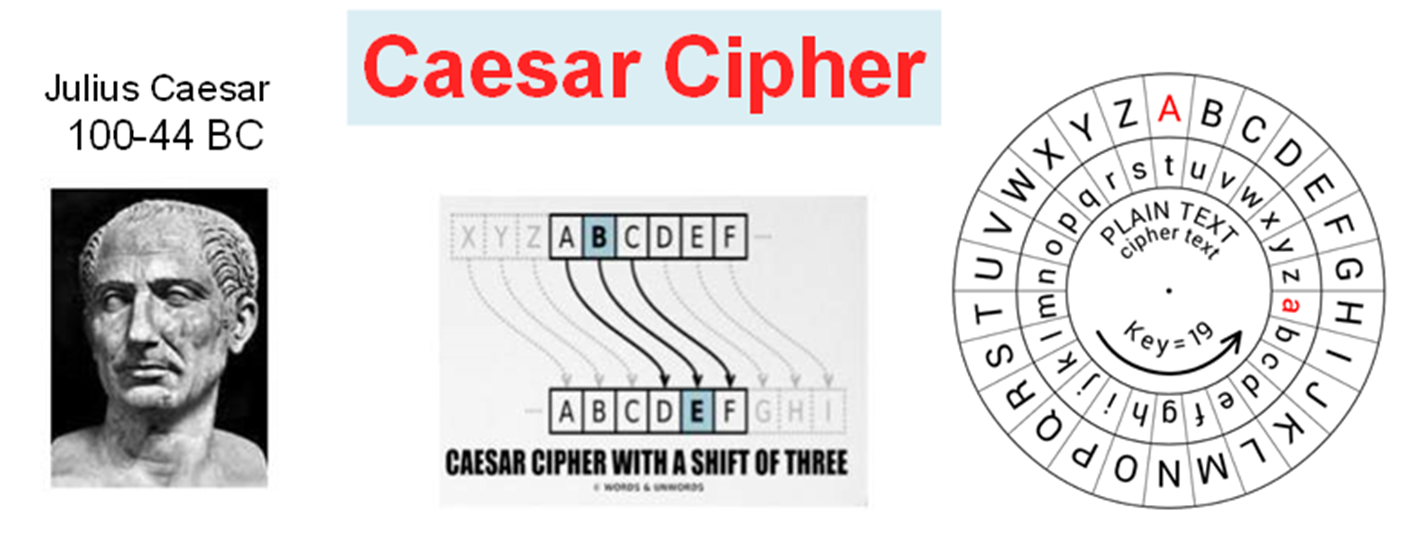
\includegraphics[angle=0, width=10.5cm]{1-crypto-practice/images/c1.png}
                \label{Figure 2}
    \end{figure}

    %\begin{center}
    %    {\Huge\calligra Enjoy!}
    %\end{center}
\end{frame}

%------------------------------------------------
\begin{frame}
    \frametitle{Приклади}
    \begin{figure}[h!]
                \centering
                % \caption{Hawkins et al, 2015}
                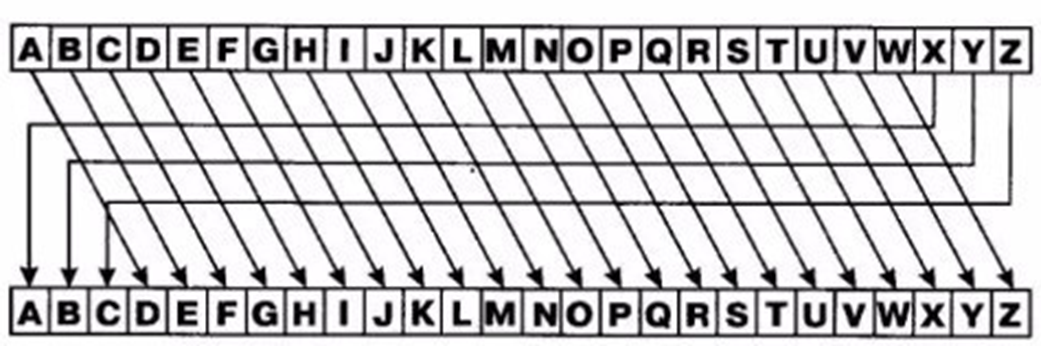
\includegraphics[angle=0, width=10.5cm]{1-crypto-practice/images/c2.png}
                \label{Figure 2}
    \end{figure}    
        	\begin{block}{Нехай задано зсув $k=3$:}
    		\textbf{Encrypt}(BAD)=EDG \\
            \vspace{5mm}
            
            \textbf{Decrypt}(EDG)=BAD
    	\end{block}
    
\end{frame}

%------------------------------------------------
\begin{frame}
    \frametitle{Математична модель}

    \begin{block}{}
        Задамо алфавіт $Z_m=\{0,1,..,m-1\}$, де $n$ -- довжина тексту. \\
        Предеставимо шифр як деяку систему $\mathcal{I}=\{\mathcal{K,M,C},\mathsf{E,D}\}$, де \\
        $\mathcal{K}$ -- ключовий простір (множина усіх ключів),\\
        $\mathcal{M}$ -- множина відкритих текстів (повідомлень),\\
        $\mathcal{C}$ -- множина зашифрованих повідомлень (шифротекстів), \\
        \texttt{E} -- функція шифрування, \\
        \textsf{D} -- функція дешифрування.
    \end{block}

    \begin{block}{}
        ВТ : $X=x_1,x_2,..,x_n\quad$ або $\quad M=m_1,m_2,..,m_n$. \\
        ШТ : $Y=y_1,y_2,..,y_n\quad$ або $\quad C=c_1,c_2,..,c_n$
    \end{block}

\end{frame}

\begin{frame}{Схема шифрування}
\begin{block}{}
    $E:\mathcal{M}\rightarrow\mathcal{C}:\quad    y_i=x_i+k \textsf{ mod } n, 1\leq i\leq n$
    
    $D:\mathcal{C}\rightarrow\mathcal{M}:\quad x_i=y_i-k \textsf{ mod } n, 1\leq i\leq n$
\end{block}
    \begin{figure}[h!]
                \centering
                % \caption{Hawkins et al, 2015}
                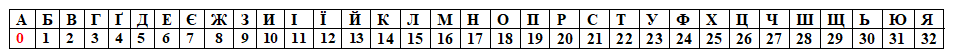
\includegraphics[angle=0, width=11.5cm]{1-crypto-practice/images/c3.png}
                \label{Figure 2}
    \end{figure} 
    \begin{block}{Задача 1.}
        Задано деяку криптограму : \textsc{ХПТСКЛЗЧЦБ}. Розшифруйте її.
    \end{block}
    \begin{alertblock}{Підказка}
        Яка потужність ключового простору $|K|=?$
    \end{alertblock}

\end{frame}

%------------------------------------------------

\begin{frame}{Частотний криптоаналіз}
     \begin{columns}[c] % [c] вирівнювання по центру вертикалі
        \column{0.5\textwidth}
        \begin{figure}
            \centering
            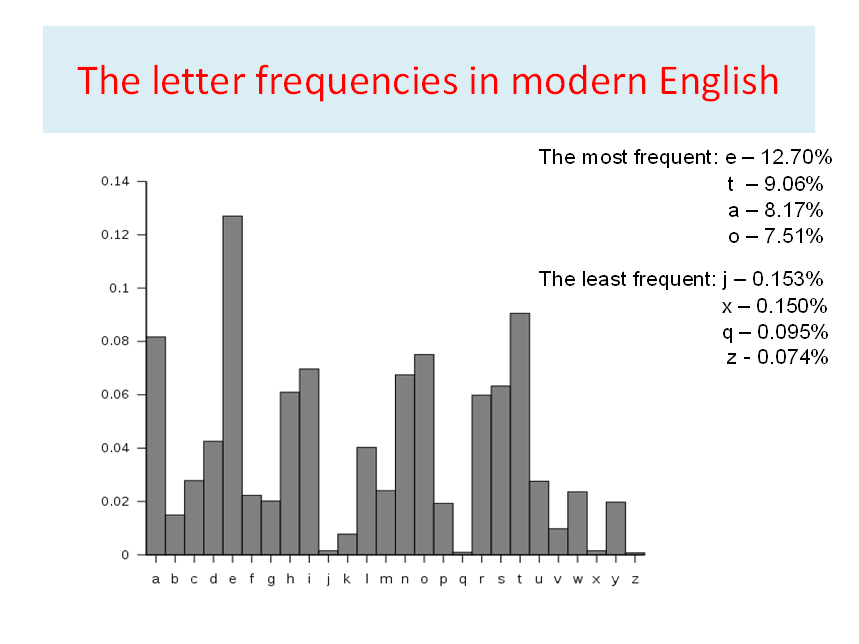
\includegraphics[width=\linewidth]{1-crypto-practice/images/f1.png}
        \end{figure}

        \column{0.5\textwidth}
        \begin{figure}
            \centering
            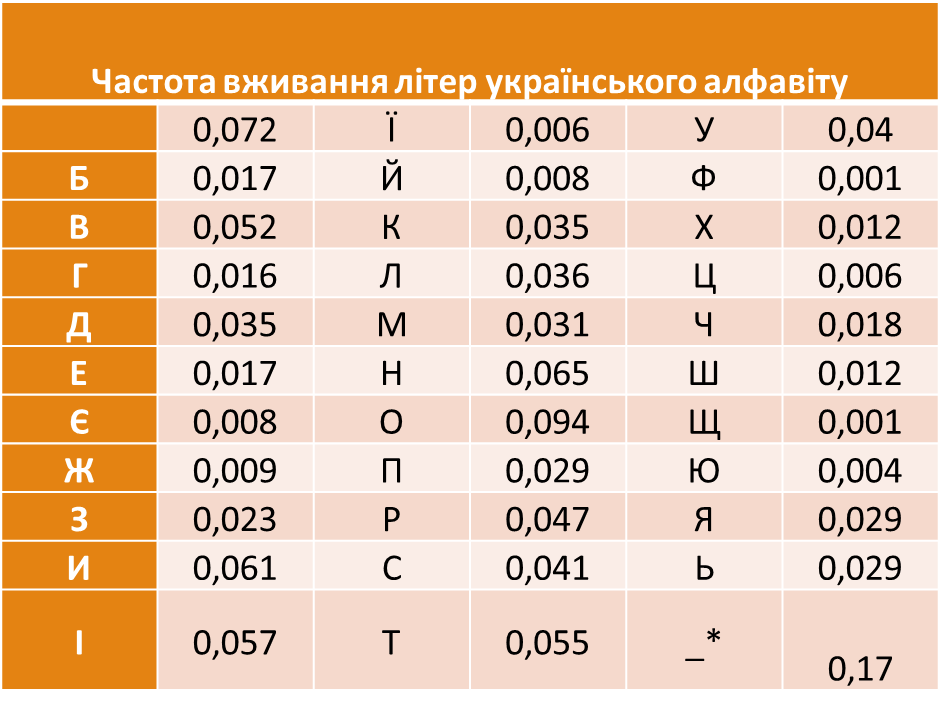
\includegraphics[width=\linewidth]{1-crypto-practice/images/f2.png}
        \end{figure}
    \end{columns}
\end{frame}

\begin{frame}
    \frametitle{Узагальнення шифру Цезаря}
    \begin{exampleblock}{Визначення}
        \textbf{\textit{Шифр зсуву}} -- перетворення, що переводить символи відкритого тексту у символи шифротексту:
        \vspace{-5mm}
        \begin{align*}
            y_i=(x_i+b)\textsf{ mod }m, \text{ де $b$ є ключем.}
        \end{align*} 
        \textbf{\textit{Лінійний шифр}} -- перетворення, що переводить символи відкритого тексту у символи шифротексту за правилом:
        \vspace{-2mm}
        \begin{align*}
            y_i=a\cdot x_i\textsf{ mod }m, \text{ де ключем є число $a\in\mathbb{Z}_m^*$}.
        \end{align*}
        Розшифрування для лінійного шифру виконується за правилом:
        \vspace{-2mm}
        \begin{align*}
            x_i=a^{-1}\cdot y_i\textsf{ mod }m.
        \end{align*}
    \end{exampleblock}
    
    
\end{frame}

%------------------------------------------------

\begin{frame}
    \frametitle{Афінний шифр. Схема}
    
    \begin{exampleblock}{Визначення}
        \textbf{\textit{Афінний шифр}} -- перетворення, що поєднує у собі лінійні шифри та шифри зсуву. Шифрування відбувається за правилом:
        \begin{align*}
            y_i=(a\cdot x_i+b) \textsf{ mod }m, \text{ де ключ це пара $(a,b), a\in\mathbb{Z}_{m}^*, b\in\mathbb{Z}_m$}.
        \end{align*}
        
    \end{exampleblock}
\end{frame}

\begin{frame}
    \frametitle{Узагальнення шифру Цезаря. Афінний шифр}
    
    \begin{exampleblock}{Визначення}
    Для роботи із лінійними та афінними шифрами потрібно вміти розв`язувати лінійні порівняння за модулем.

    Нехай $a\cdot x\equiv b (\textsf{ mod }n)$ і треба встановити значення $x$ за відомими значеннями $a,b$. Маємо наступні випадки:
    \begin{enumerate}
        \item $gcd(a,n)=1\quad\Rightarrow\quad$ маємо один розв`язок порівняння: $x\equiv a^{-1}\cdot b(\textsf{ mod }n)$.
        \item $gcd(a,n)>1\quad\Rightarrow\quad$ можливі два варіанти:
        \begin{enumerate}
            \item Якщо $b$ не ділиться на $d$, то порівняння не має розв`язків
            \item Інакше, порівняння має $d$ розв`язків виду $x_0, x_0+n_1,x_0+2n_1,..,x_0+(d-1)n_1$, де $a=a_1\cdot d$, $b=b_1\cdot d$, $n=n_1\cdot d$ і $x_0$ -- єдиний розв`язок рівняння $a_1\cdot x\equiv b_1 (\textsf{ mod }n_1)$.
        \end{enumerate}
    \end{enumerate}
    \end{exampleblock}
\end{frame}

\begin{frame}{Задачі}
\vspace{-15mm}
    \begin{figure}[h!]
                \centering
                % \caption{Hawkins et al, 2015}
                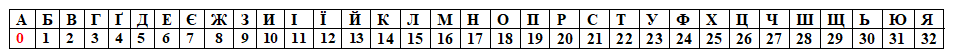
\includegraphics[angle=0, width=11.5cm]{1-crypto-practice/images/c3.png}
                \label{Figure 2}
    \end{figure} 
\begin{block}{}
\begin{enumerate}
    \item Розв`язати:
    \begin{itemize}
        \item $19^{-1}\textsf{ mod }101$
        \item $5x\equiv 13 \textsf{ mod }21$
        \item $12x\equiv 10 \textsf{ mod }162$
    \end{itemize}
    \item Розшифрувати за допомогою афінного шифру криптотекст <<КІЮИЧ>>, для $a=4,b=4$.
    \item Відомо, що шифротекст «ЩПКПИТ» одержано із відкритого тексту «КОРОЛЬ» за допомогою афінного шифру. Знайдіть ключ шифрування.
\end{enumerate}    
\end{block}
    
\end{frame}


\begin{frame}{Аналіз афінного шифру}
Нехай $x'$ -- найчастіша літера у мові, $y'$ -- найчастіша літера у шифротексті
\begin{exampleblock}{Як взламати афінний шифр}
    \begin{gather*}
        \Big\{ \begin{array}{l} 
        y'=(ax'+b)\textsf{ mod } m;  \\
        y''=(ax''+b)\textsf{ mod } m.
        \end{array} \\
        y'-y''=a(x'-x'')\textsf{ mod } m;\\
        a=( y'-y'')(x'-x'')^{-1}\textsf{ mod } m;\\
        b=y'-ax'\textsf{ mod } m.
    \end{gather*}
\end{exampleblock}
    
\end{frame}

\begin{frame}{Шифр Цезаря з автоключем}
\begin{exampleblock}{Визначення}
    Це модифікація шифру Цезаря, де перша літера відкритого тексту шифрується як в звичайному шифрі Цезаря, а всі наступні літери шифруються шляхом додавання попередніх літер відкритого тексту:
    \begin{gather*}
        c_0=(m_0+k)\textsf{ mod }n, \\
        c_i=(m_{i-1}+m_i)\textsf{ mod } n, \forall i\geq1.
    \end{gather*}
\end{exampleblock}
\begin{block}{}
    На домашнє завдання спробувати побудувати атаку з допомогою частотного криптоаналізу.
\end{block}
    
\end{frame}

\begin{frame}{Задачі}
\begin{exampleblock}{Визначення}
    Повідомлення $M$ називають нерухомою точкою шифру $E$, якщо для деякого ключа $k$ виконується $E_k(M)=M$ (звісно, що для різних ключів шифр може мати різні нерухомі точки). Такі точки є загрозливими у криптосистемах через можливі втрати конфіденційності.
\end{exampleblock}
\begin{block}{}
    \begin{enumerate}
        \item Нехай $n$ -- просте число. Доведіть, що будь-який афінний шифр при $a\neq 1$ матиме рівно одну нерухому точку 
        \item Наведіть приклад афінного шифру, який не буде мати нерухомих точок.
    \end{enumerate}
\end{block}

\end{frame}

\section{Шифр Віженера}
\begin{frame}{Шифр Віженера}
    \begin{exampleblock}{}
        Для шифрування використовується ключове слово $K=k_0k_1k_2...k_{r-1}$, що також складається із літер алфавіту $A$.
        
        \vspace{5mm}
        Процедура шифрування виконується наступним чином:
        \begin{enumerate}
            \item Доповнити ключ до довжини відкритого тексту, повторюючи його необхідну кількість разів: $K=k_0k_1...k_{r-1}k_rk_{r+1}...$, де $\forall i\geq r$ виконується рівність $k_i=k_{i\textsf{ mod }r}$;
            \item Обчислити ШТ за правилом $y_i=(x_i+k_i)\textsf{ mod }m.$
        \end{enumerate}
    \end{exampleblock}
\end{frame}

\begin{frame}{Схема}
    \begin{figure}
        \centering
        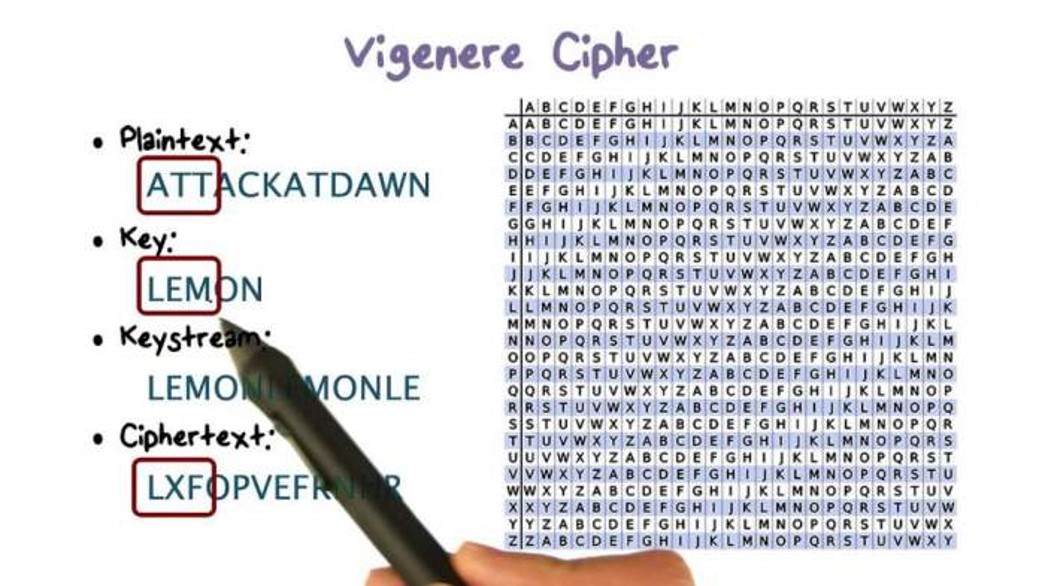
\includegraphics[width=0.8\linewidth]{1-crypto-practice/images/v1.jpg}
        \label{fig:placeholder}
    \end{figure}
\end{frame}

\begin{frame}{Шифр Віженера з автоключем}
    \begin{exampleblock}{Визначення}
        Модифікація шифру Віженера, де в якості ключової послідовності використовується той самий ВТ, тобто, в ключовій послідовності після ключ записуються символи ВТ:
        \begin{align*}
            K=k_0k_1k_2...k_{r-1}x_0x_1,
        \end{align*} або,іншими словами, для кожного $i \geq r$ виконується рівність: $k_i=x_i-r$
    \end{exampleblock}
\end{frame}

\begin{frame}{Задачі}
\vspace{-9mm}
    \begin{block}{}
        \begin{figure}[h!]
                \centering
                % \caption{Hawkins et al, 2015}
                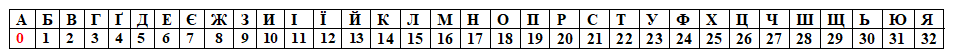
\includegraphics[angle=0, width=10.5cm]{1-crypto-practice/images/c3.png}
                \label{Figure 2}
    \end{figure} 
    \begin{enumerate}
        \item  \begin{itemize}
            \item Зашифруйте повідомлення <<ПЕРСТЕНЬНЕСЕФРОДО>> шифром Віженера із ключем <<САУРОН>>.
            \item Зашифруйте те саме повідомлення тим самим ключем, але використовуючи шифр Віженера із автоключем.
        \end{itemize}
        \item Розширфувати криптограму <<ЬУЧОЬОТ>>, зашифровану шифром Віженера із ключем <<КАВА>>.
        \item Нехай алфавіт $A$ містить $m$ символів. Яку потужність має ключовий простір афінного шифру? шифру Віженера із довжиною ключа $r$? шифру Віженера із довжиною ключа не більше $r$?
    \end{enumerate}
\end{block}
\end{frame}

    \begin{frame}[plain, standout]
    \begin{figure}
        \centering
        
\includegraphics[width=0.9\linewidth]{Cryptocats.jpg}
        \label{fig:placeholder}
    \end{figure}
    \centering
    \LARGE
    \textbf{Питання?} \\

    \vspace{0.2cm} \Huge \ding{170} \large \\

  \end{frame}
\end{document}